\documentclass[conference]{IEEEtran}

\IEEEoverridecommandlockouts

\usepackage{cite}
\usepackage{amsmath,amssymb,amsfonts}
\usepackage{amsthm}
\newtheorem{lemma}{Lemma}
\newtheorem{proposition}{Proposition}
\newtheorem{remark}{Remark}
\usepackage{graphicx}
\usepackage{textcomp}
\usepackage{xcolor}
\usepackage{url}
\usepackage[hidelinks]{hyperref}
\usepackage{algorithm}
\usepackage{algorithmic}

\title{Adaptive Sampling for Chamfer Distance Estimation}

\author{
\IEEEauthorblockN{Cody Jiang}
\IEEEauthorblockA{
New York University\\
cody.jiang@nyu.edu}
\and
\IEEEauthorblockN{Yifan Hu}
\IEEEauthorblockA{
New York University\\
yh6416@nyu.edu}
}

\begin{document}

\maketitle

\begin{center}
\small
Code and data: \url{https://github.com/whohyf/Adaptive-Sampling-for-Chamfer-Distance-Estimation.git}
\end{center}

\begin{abstract}
The Chamfer distance between two point sets $A, B \subset \mathbb{R}^d$
is a widely used dissimilarity measure for point clouds and document
embeddings, but the naive estimator runs in $O(n^2 d)$ time. Bakshi
et al.\ (2023) gave the first $(1{+}\varepsilon)$-approximate estimator
running in $O(nd \log(n)/\varepsilon^2)$ time, based on importance
sampling driven by a coarse-nearest-neighbor preprocessing step
(\textsc{CrudeNN}). A simpler uniform-sampling baseline avoids the
preprocessing entirely but requires
$O(\mathrm{CV}^2(\gamma)/\varepsilon^2)$ samples, where
$\mathrm{CV}(\gamma)$ is the coefficient of variation of the per-point
nearest-neighbor distances --- a quantity that is not available
without substantial work. We re-implement both estimators, reproducing
the qualitative behavior of Bakshi et al.\ and matching their
\textsc{CrudeNN} quality trend quantitatively
(e.g., expansion ratio $2.30$ at three LSH levels versus the paper's
$\approx 2.0$). We then study whether a small uniform pilot can
support an automatic choice between uniform sampling and importance
sampling. On a $162$-instance benchmark, a pilot of size $50$
estimates $\mathrm{CV}(\gamma)$ within $30\%$ of its true value on
$80\%$ of instances. However, threshold sweeps show that the regime
boundary remains genuinely difficult: near the break-even region, the
default pilot rule incurs a $15\%$ false-positive rate and a $50\%$
false-negative rate. End-to-end, the adaptive rule nearly matches
uniform on low-CV text-like data and reaches IS-level error on our
ShapeNet-like setting, while a planted-outlier dataset exposes a
different limitation: at small $n$, cost-based routing and estimation
quality can point in different directions. These results suggest that
a pilot-based rule is useful as a practical heuristic, but does not
eliminate uncertainty near the sampling-regime boundary.
\end{abstract}

\section{Introduction}
\label{sec:intro}

The Chamfer distance from $A$ to $B$ is
$\mathrm{CH}(A, B) = \sum_{a \in A} \min_{b \in B} d(a, b)$,
where $d$ is typically the $\ell_1$ or $\ell_2$ distance. It is a
standard dissimilarity measure between point clouds in computer vision,
graphics, and robotics, and serves as a tractable relaxation of the
Earth Mover's Distance in document-similarity applications, where
points are word embeddings and $\mathrm{CH}(A, B)$ measures the cost of
matching each word in document $A$ to its closest counterpart in
document $B$~\cite{kusner2015wmd}. It also appears as a training
objective for neural implicit surface fitting and other learned
geometry pipelines~\cite{diffcd2024}. Implementations are shipped in
TensorFlow Graphics, PyTorch3D, and PDAL. Because $\mathrm{CH}(A, B)$
is a sum of $n$ nearest-neighbor distances, the naive estimator costs
$O(n^2 d)$ time; on the large-scale datasets that motivate modern
applications, this quadratic dependence is prohibitive.

Bakshi et al.~\cite{bakshi2023near} resolved the asymptotic question by
giving the first $(1{+}\varepsilon)$-approximate estimator with
near-linear running time, $O(nd \log(n)/\varepsilon^2)$. Their
algorithm has two stages. A preprocessing step, \textsc{CrudeNN}, uses
$O(\log n)$ levels of randomly shifted grid hashing to produce, for
each $a \in A$, an estimate $D_a$ that deterministically upper-bounds
the true nearest-neighbor distance
$\gamma_a = \min_{b \in B} d(a, b)$ and satisfies
$\mathbb{E}[D_a] \leq O(\log n) \cdot \gamma_a$. The estimator
\textsc{Chamfer-Estimate} then draws $T = O(\log(n)/\varepsilon^2)$
samples from $A$ with probability proportional to $D_a$ and outputs
the corresponding importance-sampling average. Feng and
Indyk~\cite{feng2025faster} subsequently improve the asymptotic
complexity further; the present paper is concerned with a practical
question that remains even if the asymptotics improve: \emph{when is
the importance-sampling machinery actually worth using?}

That question arises because the simplest competing estimator ---
uniform sampling without preprocessing --- can be much cheaper on
low-variance data. Its sample complexity scales as
$O((1+\mathrm{CV}^2(\gamma))/\varepsilon^2)$, where
$\mathrm{CV}(\gamma) = \sigma(\gamma)/\mu(\gamma)$ is the coefficient
of variation of the per-point nearest-neighbor distances $\gamma_a$.
Comparing this against the $O(nd \log n)$ preprocessing overhead of
\textsc{CrudeNN}, the asymptotic break-even occurs around
$\mathrm{CV}^2(\gamma) \asymp \log n$: below this threshold, uniform
sampling benefits from skipping preprocessing; above it, the variance
of uniform sampling can become prohibitive and importance sampling
becomes attractive. The user therefore faces a choice between two
estimators whose relative cost depends on a latent property of the
input distribution.

The difficulty, of course, is that $\mathrm{CV}(\gamma)$ is not given
for free. Estimating it exactly requires computing all nearest-neighbor
distances, which largely defeats the purpose of using a sub-quadratic
estimator in the first place. This circularity suggests a natural
workaround: draw a small uniform pilot, compute the corresponding
$\gamma$ values exactly, estimate $\mathrm{CV}(\gamma)$ from that
pilot, and route to either a uniform or an importance-sampling branch.
Because the pilot points are themselves valid uniform samples, they can
also be reused if the rule selects the uniform path.

The present work asks how far this workaround actually goes in
practice. Three questions matter. First, how accurately can a small
pilot estimate $\mathrm{CV}(\gamma)$ across a range of data
distributions? Second, how sensitive is the branch decision to the
threshold used to convert $\widehat{\mathrm{CV}}$ into a routing rule?
Third, when evaluated end-to-end, does a pilot-based adaptive rule
actually behave like the better of the two pure estimators, or does it
merely shift the decision problem into a noisy preprocessing step? Our
experiments show a mixed answer: pilot calibration is often good on
easy instances, but the regime boundary remains genuinely hard, and
heavy-tailed data exposes a deeper limitation than simple threshold
miscalibration.

\textbf{Contributions.}
\begin{itemize}
    \item \textbf{A faithful re-implementation of the Bakshi et al.\
    estimator.} We re-implement \textsc{CrudeNN} and
    \textsc{Chamfer-Estimate} from scratch and reproduce
    Figures~3, 4, and 6(b) of the original paper. The reproduction is
    qualitative on Figures~3 and~4 and quantitative on Figure~6(b):
    at three LSH levels, our mean \textsc{CrudeNN} expansion ratio is
    $2.30$, compared with the paper's $\approx 2.0$. We also identify
    implementation choices that materially affect practical behavior,
    including dataset calibration and a vectorized \textsc{CrudeNN}
    implementation that substantially reduces preprocessing cost in
    Python.

    \item \textbf{An empirical characterization of pilot calibration
    and the regime boundary.} Combining the standard Chebyshev bound
    for uniform sampling with Lemma~2.2 of Bakshi et al., the
    asymptotic break-even sits at
    $\mathrm{CV}^2(\gamma) \asymp \log n$. On a $162$-instance
    benchmark, a pilot of size $s=50$ estimates
    $\mathrm{CV}(\gamma)$ within $30\%$ of its true value on
    $80\%$ of instances. At the same time, threshold sweeps show that
    borderline instances remain difficult: near the break-even region,
    the default pilot rule incurs a $15\%$ false-positive rate and a
    $50\%$ false-negative rate on the borderline subset.

    \item \textbf{An adaptive estimator and an honest end-to-end
    evaluation.} We implement \textsc{Adaptive-Chamfer}, which uses a
    uniform pilot to choose between uniform sampling and importance
    sampling. On low-CV text-like data, the rule correctly collapses to
    the uniform path and nearly matches its cost and error. On our
    ShapeNet-like setting, it reaches IS-level mean estimation error,
    although pure IS is slightly lower in the canonical run. On a
    planted-outlier dataset, however, the experiments expose a
    different limitation: at small
    $n$, cost-based routing can still favor the uniform/brute-force side
    even though estimation quality is poor, so the pilot does not
    resolve the regime boundary as much as reveal it.
\end{itemize}

The rest of the paper proceeds in that order. Section~\ref{sec:background}
reviews the Bakshi et al.\ algorithm and the implementation choices
behind our reproduction. Section~\ref{sec:theory} works out the
variance bounds for both estimators, the resulting break-even, and the
bias of the sample-CV estimator. Section~\ref{sec:algorithm} states
\textsc{Adaptive-Chamfer} and discusses the threshold-based decision
rule together with its heavy-tail failure mode. Section~\ref{sec:experiments}
reports the reproduction, calibration, threshold, and end-to-end
results. Section~\ref{sec:discussion} discusses the limits of
pilot-based routing and possible directions for more robust statistics.



\section{Background}
\label{sec:background}

\subsection{Problem and Notation}
\label{sec:problem}

For two finite point sets $A, B \subset \mathbb{R}^d$ with
$|A|, |B| \leq n$, the (one-sided) Chamfer distance from $A$ to $B$
under a metric $d_X$ is
\begin{equation}
    \mathrm{CH}(A, B) = \sum_{a \in A} \min_{b \in B} d_X(a, b)
                     = \sum_{a \in A} \gamma_a,
\label{eq:chamfer}
\end{equation}
where $\gamma_a := \min_{b \in B} d_X(a, b)$ denotes the
nearest-neighbor distance from $a$ to $B$. Throughout the paper we
take $d_X$ to be either the $\ell_1$ or the $\ell_2$ distance. The
symmetric Chamfer distance is
$\mathrm{CH}(A, B) + \mathrm{CH}(B, A)$ and is estimated by running
the one-sided estimator twice; we focus on the one-sided case in the
analysis. Let
\begin{equation}
    \mu  := \tfrac{1}{n} \sum_{a \in A} \gamma_a, \qquad
    \sigma^2 := \tfrac{1}{n} \sum_{a \in A} (\gamma_a - \mu)^2,
\label{eq:moments}
\end{equation}
and define the coefficient of variation
$\mathrm{CV}(\gamma) := \sigma / \mu$. The naive estimator computes
$\gamma_a$ for every $a \in A$ and runs in $O(n^2 d)$ time. The
approximate estimators studied below are designed to avoid the
quadratic brute-force computation by replacing the full sum with either
uniform or importance-weighted nearest-neighbor queries. We nevertheless
retain brute force as a baseline, and the adaptive method may
deliberately fall back to exact computation when the conservative
uniform-sampling budget reaches $n$.

\subsection{The Bakshi et al.\ Estimator}
\label{sec:bakshi-summary}

The estimator of Bakshi et al.~\cite{bakshi2023near} is built from two
subroutines: a coarse nearest-neighbor preprocessing step
\textsc{CrudeNN} (Algorithm~\ref{alg:crudenn}), and an importance-sampling
estimator \textsc{Chamfer-Estimate} (Algorithm~\ref{alg:cest}) that
consumes the output of the first.

\begin{algorithm}[t]
\caption{$\textsc{CrudeNN}(A, B)$ for the $\ell_1$ metric}
\label{alg:crudenn}
\begin{algorithmic}[1]
\REQUIRE $A, B \subset \mathbb{R}^d$ with all nonzero pairwise
distances in $[1, \mathrm{poly}(n/\varepsilon)]$.
\ENSURE $\{D_a\}_{a \in A}$ with $D_a \geq \gamma_a$ deterministically
        and $\mathbb{E}[D_a] \leq O(\log n) \cdot \gamma_a$.
\STATE Set $L \gets O(\log(n/\varepsilon))$ and $r_i \gets 2^i$ for
       $i = 0, \dots, L$.
\STATE For each $i$, sample a shift $z^{(i)} \sim [0, r_i]^d$ and
       define the hash $h_i(x) = \lfloor (x + z^{(i)}) / r_i \rfloor$
       (componentwise).
\STATE Hash all $b \in B$ at every level $i$ and store
       $\{(h_i(b), b)\}$.
\FOR{each $a \in A$}
    \STATE Find the smallest $i^* \in \{0, \dots, L\}$ for which there
           exists $b' \in B$ with $h_{i^*}(a) = h_{i^*}(b')$.
    \STATE Set $D_a \gets \|a - b'\|_1$.
\ENDFOR
\end{algorithmic}
\end{algorithm}

\textsc{CrudeNN} is a multi-scale locality-sensitive hash family
(see Bakshi et al.~\cite{bakshi2023near}, Definition~A.1): at each
scale $r_i$, close points $x, y$ fail to collide under $h_i$ with
probability at most $\|x - y\|_1 / r_i$, while far points collide
with probability at most $\exp(-c_1 \|x - y\|_1 / r_i)$ for an
absolute constant $c_1 > 0$. Scanning levels from finest ($i = 0$) to
coarsest ($i = L$) and stopping at the first collision gives the two
properties annotated in Algorithm~\ref{alg:crudenn}: $D_a$ is always
the $\ell_1$ distance from $a$ to some actual point in $B$ (so
$D_a \geq \gamma_a$ holds with probability $1$), and the expected
collision scale exceeds $\gamma_a$ by at most an $O(\log n)$ factor.
For the $\ell_2$ metric, a Johnson--Lindenstrauss projection embeds
$A \cup B$ into $\mathbb{R}^k$ with $k = O(\log n / \varepsilon^2)$,
preserving all pairwise distances up to $(1 \pm \varepsilon)$, and the
$\ell_1$ version is then applied. The total running time of
\textsc{CrudeNN} is $O(nd \log(n/\varepsilon))$.

\begin{algorithm}[t]
\caption{$\textsc{Chamfer-Estimate}(A, B, T)$}
\label{alg:cest}
\begin{algorithmic}[1]
\REQUIRE $A, B \subset \mathbb{R}^d$ and a sample budget $T \in \mathbb{N}$.
\ENSURE An estimate $\eta$ of $\mathrm{CH}(A, B)$.
\STATE $\{D_a\}_{a \in A} \gets \textsc{CrudeNN}(A, B)$;\quad
       $D \gets \sum_{a \in A} D_a$.
\STATE Define the distribution $\mathcal{D}$ on $A$ by
       $\Pr_{x \sim \mathcal{D}}[x = a] := D_a / D$.
\FOR{$\ell = 1, \dots, T$}
    \STATE Sample $x_\ell \sim \mathcal{D}$ and compute exactly
           $\gamma_{x_\ell} = \min_{b \in B} \|x_\ell - b\|_1$.
    \STATE $\eta_\ell \gets (D / D_{x_\ell}) \cdot \gamma_{x_\ell}$.
\ENDFOR
\STATE \textbf{return} $\eta \gets \tfrac{1}{T} \sum_{\ell=1}^T \eta_\ell$.
\end{algorithmic}
\end{algorithm}

\textsc{Chamfer-Estimate} is a standard importance-sampling
construction with the proposal $\mathcal{D}$ chosen so that points
contributing more to $\mathrm{CH}(A, B)$ are sampled more often.
Unbiasedness follows directly from the choice of $\mathcal{D}$:
$\mathbb{E}[\eta_\ell] = \sum_a (D_a / D)(D / D_a) \gamma_a
= \mathrm{CH}(A, B)$. The non-trivial part is the variance bound,
which we restate from~\cite{bakshi2023near} for use in
Section~\ref{sec:theory}.

\begin{lemma}[Bakshi et al.\ \cite{bakshi2023near}, Lemma 2.2]
\label{lem:is-variance}
For any $T \in \mathbb{N}$, the output $\eta$ of
$\textsc{Chamfer-Estimate}(A, B, T)$ satisfies
$\mathbb{E}[\eta] = \mathrm{CH}(A, B)$ and
\begin{equation}
    \mathrm{Var}[\eta] \leq
    \frac{\mathrm{CH}(A, B)^2}{T}
    \left( \frac{D}{\mathrm{CH}(A, B)} - 1 \right).
\label{eq:is-variance}
\end{equation}
In particular, by Chebyshev's inequality,
\begin{multline}
\Pr\!\left[
|\eta-\mathrm{CH}(A,B)|
\ge
\varepsilon\mathrm{CH}(A,B)
\right] \\
\le
\frac{1}{\varepsilon^2T}
\left(
\frac{D}{\mathrm{CH}(A,B)}-1
\right).
\label{eq:is-chebyshev}
\end{multline}
\end{lemma}

The upper-bound property of \textsc{CrudeNN} guarantees
$D \leq O(\log n) \cdot \mathrm{CH}(A, B)$ in expectation, so setting
$T = O(\log(n) / \varepsilon^2)$ in Lemma~\ref{lem:is-variance} suffices
for $(1 \pm \varepsilon)$ relative error with constant probability.
Combined with the $O(nd \log(n/\varepsilon))$ cost of \textsc{CrudeNN}
and the $O(nd)$ cost of each exact nearest-neighbor query in
Algorithm~\ref{alg:cest} line~4, the total running time is
$O(nd \log(n) / \varepsilon^2)$. A subsequent result by Feng and
Indyk~\cite{feng2025faster} improves the $\log n$ factor; both results
share the same two-stage structure and the same dependence on
$\textsc{CrudeNN}$-style preprocessing, so the practical question
studied in this paper applies to both.

\section{Variance Analysis: \\ Uniform vs.\ Importance Sampling}
\label{sec:theory}

This section compares uniform sampling and importance sampling in a
common cost model. We first give a distribution-free Chebyshev bound
for the uniform estimator; this is the bound used by the runtime
uniform path of \textsc{Adaptive-Chamfer}. We then give a Bernstein
refinement under a bounded-ratio condition
$\gamma_a/\mu \leq M$, which is substantially sharper on well-behaved
instances. The Bernstein bound is used as the reference oracle in our
FP/FN analysis, while the runtime algorithm keeps the Chebyshev budget
for its uniform branch. Finally, we discuss the difficulty of estimating
the relevant pilot statistics from a small uniform sample.

\subsection{Uniform Sampling Variance}
\label{sec:unif-variance}

The uniform-sampling estimator draws indices
$x_1, \dots, x_T$ independently and uniformly from $A$, computes
$\gamma_{x_i}$ exactly for each, and outputs
\begin{equation}
    \widehat{\mathrm{CH}}_U
    := \frac{n}{T} \sum_{i=1}^{T} \gamma_{x_i}.
\label{eq:unif-est}
\end{equation}
Unbiasedness is immediate:
$\mathbb{E}[\widehat{\mathrm{CH}}_U]
= \frac{n}{T} \cdot T \cdot \frac{1}{n} \sum_{a \in A} \gamma_a
= \mathrm{CH}(A, B)$. For the variance, each summand $\gamma_{x_i}$
has variance $\sigma^2$ (cf.~Eq.~\ref{eq:moments}) under the uniform
draw, and the $n/T$ rescaling gives
\begin{equation}
    \mathrm{Var}\!\left[\widehat{\mathrm{CH}}_U\right]
    = \frac{n^2 \sigma^2}{T}
    = \frac{\mathrm{CH}(A, B)^2 \cdot \mathrm{CV}^2(\gamma)}{T},
\label{eq:unif-variance}
\end{equation}
where the second equality uses
$\mathrm{CH}(A, B) = n \mu$ and
$\mathrm{CV}^2(\gamma) = \sigma^2 / \mu^2$. Equation~\ref{eq:unif-variance}
is the form we will use throughout: the relative variance of the
uniform estimator is exactly $\mathrm{CV}^2(\gamma) / T$. Applying
Chebyshev's inequality gives the relative-error guarantee.

\paragraph{Sampling convention.}
For notational simplicity, the variance calculations in this section
analyze the uniform estimator under independent sampling with replacement.
The implementation, including the pilot stage of
\textsc{Adaptive-Chamfer}, samples without replacement whenever the requested
budget is at most $n$. This only reduces the sampling variance through the
usual finite-population correction, so the with-replacement bounds used here
remain conservative for the implemented estimator. We therefore use the
i.i.d.\ analysis as a clean upper-bound model while reporting the actual
without-replacement implementation in the algorithms and experiments.

\begin{proposition}[Uniform sampling Chebyshev bound]
\label{prop:unif-cheb}
For any $\varepsilon \in (0, 1)$ and $T \geq 1$,
\begin{equation}
    \Pr\!\left[\, \big|\widehat{\mathrm{CH}}_U - \mathrm{CH}(A, B)\big|
    \geq \varepsilon \cdot \mathrm{CH}(A, B) \,\right]
    \leq \frac{\mathrm{CV}^2(\gamma)}{\varepsilon^2 \, T}.
\label{eq:unif-cheb}
\end{equation}
In particular, $T_\mathrm{unif}
= \lceil \mathrm{CV}^2(\gamma) / (\varepsilon^2 \delta) \rceil$
samples suffice for $(1 \pm \varepsilon)$ relative error with
probability at least $1 - \delta$.
\end{proposition}

\begin{proof}
Apply Chebyshev's inequality to
$\widehat{\mathrm{CH}}_U$ using
Eq.~\ref{eq:unif-variance}:
\[
\Pr\!\left[
    \left|
        \widehat{\mathrm{CH}}_U - \mathrm{CH}
    \right|
    \geq
    \varepsilon \mathrm{CH}
\right]
\leq
\frac{
    \mathrm{Var}[\widehat{\mathrm{CH}}_U]
}{
    (\varepsilon \mathrm{CH})^2
}
=
\frac{
    \mathrm{CV}^2(\gamma)
}{
    \varepsilon^2 T
}.
\]
\end{proof}

\begin{proposition}[Uniform sampling Bernstein bound]
\label{prop:unif-bernstein}
Assume $\mathrm{CH}(A,B)>0$ and define
\[
    M(\gamma) := \frac{\max_{a \in A}\gamma_a}{\mu}.
\]
If $\gamma_a/\mu \leq M(\gamma)$ for all $a \in A$, then the uniform
sampling estimator satisfies
\begin{equation}
    \Pr\!\left[
        \big|\widehat{\mathrm{CH}}_U-\mathrm{CH}(A,B)\big|
        \geq \varepsilon \mathrm{CH}(A,B)
    \right]
    \leq
    2\exp\!\left(
        -\frac{
            T\varepsilon^2
        }{
            2\left(\mathrm{CV}^2(\gamma)+M(\gamma)\varepsilon/3\right)
        }
    \right).
\label{eq:unif-bernstein-tail}
\end{equation}
Consequently,
\begin{equation}
    T_U^{\mathrm{Bern}}
    =
    \left\lceil
        \frac{
            2\left(\mathrm{CV}^2(\gamma)+M(\gamma)\varepsilon/3\right)
            \log(2/\delta)
        }{
            \varepsilon^2
        }
    \right\rceil
\label{eq:unif-bernstein-budget}
\end{equation}
samples suffice for $(1\pm\varepsilon)$ relative error with probability
at least $1-\delta$.
\end{proposition}

\begin{proof}
Let
\[
    Z_i := n\gamma_{x_i},
    \qquad
    \widehat{\mathrm{CH}}_U = \frac{1}{T}\sum_{i=1}^T Z_i .
\]
Then
\[
    \mathbb{E}[Z_i] = n\mu = \mathrm{CH}(A,B)
\]
and
\[
    \mathrm{Var}(Z_i)
    =
    n^2\sigma^2
    =
    \mathrm{CH}(A,B)^2\mathrm{CV}^2(\gamma).
\]
Moreover,
\[
    |Z_i-\mathbb{E}Z_i|
    \leq
    n\mu M(\gamma)
    =
    \mathrm{CH}(A,B)M(\gamma).
\]
Bernstein's inequality gives
\[
\Pr\!\left[
    \left|
    \frac{1}{T}\sum_{i=1}^{T}Z_i-\mathbb{E}Z_i
    \right|
    \geq t
\right]
\leq
2\exp\!\left(
    -\frac{Tt^2/2}{V+Rt/3}
\right),
\]
where
\[
    V=\mathrm{CH}(A,B)^2\mathrm{CV}^2(\gamma),
    \qquad
    R=\mathrm{CH}(A,B)M(\gamma).
\]
Setting $t=\varepsilon\mathrm{CH}(A,B)$ yields
Eq.~\ref{eq:unif-bernstein-tail}. Solving the right-hand side
for probability at most $\delta$ gives
Eq.~\ref{eq:unif-bernstein-budget}.
\end{proof}

The Bernstein bound replaces the $1/\delta$ dependence of Chebyshev
by $\log(1/\delta)$, but it pays an additional bounded-ratio term
$M(\gamma)\varepsilon/3$. It is therefore sharper precisely when the
nearest-neighbor distance distribution is not too heavy-tailed. In
particular,
\[
\frac{
    T_U^{\mathrm{Bern}}
}{
    T_U^{\mathrm{Cheb}}
}
=
2\delta\log(2/\delta)
\left(
    1+
    \frac{M(\gamma)\varepsilon}{3\mathrm{CV}^2(\gamma)}
\right),
\]
so for $\delta=0.01$ the leading factor is about $0.106$, giving an
order-of-magnitude improvement when
$M(\gamma)\varepsilon=O(\mathrm{CV}^2(\gamma))$.

The data-dependent factor $\mathrm{CV}^2(\gamma)$ is sharp: when the
$\gamma_a$ values are nearly constant, $\mathrm{CV} \to 0$ and the
required sample size collapses to a small data-independent constant;
when one or a few points dominate the sum, $\mathrm{CV}^2$ scales as
$\Theta(n)$ and Proposition~\ref{prop:unif-cheb} requires
$T_\mathrm{unif} = \Theta(n)$, defeating the purpose of sampling.

\subsection{Importance Sampling Variance}
\label{sec:is-variance}

The importance-sampling estimator $\widehat{\mathrm{CH}}_{IS} := \eta$
of Algorithm~\ref{alg:cest} satisfies
Lemma~\ref{lem:is-variance}, which we restate informally:
$\mathrm{Var}[\eta] \leq T^{-1} \mathrm{CH}(A, B)^2 (D / \mathrm{CH}(A, B) - 1)$
where $D = \sum_{a \in A} D_a$. Define the proposal-quality ratio
\begin{equation}
    \lambda := \frac{D}{\mathrm{CH}(A, B)}
    = \frac{\sum_{a \in A} D_a}{\sum_{a \in A} \gamma_a}.
\label{eq:lambda-def}
\end{equation}
Because \textsc{CrudeNN} guarantees $D_a \geq \gamma_a$ for every $a$,
we always have $\lambda \geq 1$; the closer $\lambda$ is to $1$, the
closer the IS proposal is to the optimal (oracle) proposal
$\Pr[x = a] \propto \gamma_a$. Lemma~\ref{lem:is-variance} can then
be rewritten as
\begin{equation}
    \frac{\mathrm{Var}[\widehat{\mathrm{CH}}_{IS}]}{\mathrm{CH}(A, B)^2}
    \leq \frac{\lambda - 1}{T},
\label{eq:is-rel-variance}
\end{equation}
the IS counterpart to the relative-variance form
$\mathrm{CV}^2(\gamma) / T$ from Section~\ref{sec:unif-variance}.

The two relative-variance expressions are directly comparable. The
uniform estimator's variance is governed by the data property
$\mathrm{CV}^2(\gamma)$, which can be arbitrarily large; the IS
estimator's variance is governed by $\lambda - 1$, which is bounded
in expectation regardless of the data.

\begin{proposition}[IS Chebyshev bound and sample complexity]
\label{prop:is-cheb}
With $\lambda$ as in Eq.~\ref{eq:lambda-def}, the output $\eta$ of
$\textsc{Chamfer-Estimate}(A, B, T)$ satisfies
\begin{equation}
    \Pr\!\left[\, |\eta - \mathrm{CH}(A, B)| \geq
    \varepsilon \cdot \mathrm{CH}(A, B) \,\right]
    \leq \frac{\lambda - 1}{\varepsilon^2 \, T}.
\label{eq:is-cheb}
\end{equation}
Furthermore, with probability at least $99/100$ over the randomness of
\textsc{CrudeNN}, $\lambda = O(\log n)$, so
$T_{IS} = O(\log(n) / \varepsilon^2)$ samples suffice for
$(1 \pm \varepsilon)$ relative error with constant probability.
\end{proposition}

\begin{proof}
The Chebyshev bound is the relative-variance form of
Lemma~\ref{lem:is-variance}, restated using
$\lambda = D/\mathrm{CH}(A, B)$. For the second statement, the
\textsc{CrudeNN} guarantee
$\mathbb{E}[D_a] \leq c \log n \cdot \gamma_a$ (some absolute
constant $c$) gives, by linearity,
$\mathbb{E}[D] \leq c \log n \cdot \mathrm{CH}(A, B)$. Markov's
inequality applied to $D$ yields $D \leq 100 c \log n \cdot \mathrm{CH}(A, B)$
with probability at least $99/100$, so $\lambda - 1 = O(\log n)$ on
that event. Plugging this into Eq.~\ref{eq:is-cheb} and solving
$T_{IS} \cdot \varepsilon^2 = \Omega(\log n)$ gives the claim.
\end{proof}

\subsection{Break-Even Condition}
\label{sec:break-even}

The Chebyshev and Bernstein bounds play different roles in this paper.
The Chebyshev budget is the runtime guarantee used by the uniform branch:
\begin{equation}
    T_U^{\mathrm{Cheb}}
    =
    \left\lceil
        \frac{\mathrm{CV}^2(\gamma)}{\varepsilon^2\delta}
    \right\rceil .
\label{eq:cheb-runtime-budget}
\end{equation}
This bound is distribution-free, but for the default $\delta=0.01$ it
can be pessimistic enough that brute force is cheaper than uniform
sampling on small instances. For deciding which branch an oracle would
prefer, we therefore use the Bernstein cost model
\begin{equation}
    \mathcal{C}_U^{\mathrm{Bern}}
    :=
    \min\!\left\{
        \frac{
            2\left(\mathrm{CV}^2(\gamma)+M(\gamma)\varepsilon/3\right)
            \log(2/\delta)
        }{
            \varepsilon^2
        },
        n
    \right\}.
\label{eq:cost-unif-bern}
\end{equation}
The minimum enforces the brute-force fallback: once the requested
uniform budget reaches $n$, the exact computation is no more expensive
in nearest-neighbor-query units.

For the IS path, we use the fixed-success-probability budget inherited
from \textsc{Chamfer-Estimate}:
\begin{equation}
    T_{IS}
    =
    \left\lceil
        C_{IS}\frac{\log n}{\varepsilon^2}
    \right\rceil ,
    \qquad C_{IS}=4
    \quad\text{in our experiments}.
\label{eq:is-runtime-budget}
\end{equation}
Its cost model is
\begin{equation}
    \mathcal{C}_{IS}
    :=
    C_{\mathrm{NN}}\log n
    +
    C_{IS}\frac{\log n}{\varepsilon^2},
\label{eq:cost-is-oracle}
\end{equation}
where the first term represents \textsc{CrudeNN} preprocessing and the
second term represents exact nearest-neighbor evaluations for sampled
points.

Equating Eq.~\ref{eq:cost-unif-bern} and Eq.~\ref{eq:cost-is-oracle}
gives the Bernstein oracle's break-even condition:
\begin{equation}
    \mathrm{CV}^2(\gamma)+M(\gamma)\varepsilon/3
    \approx
    \frac{\varepsilon^2}{2\log(2/\delta)}
    \left(
        C_{\mathrm{NN}}\log n
        +
        C_{IS}\frac{\log n}{\varepsilon^2}
    \right).
\label{eq:bernstein-break-even}
\end{equation}
For fixed $\varepsilon,\delta,C_{\mathrm{NN}}$, and $C_{IS}$, this is
still a logarithmic break-even. In the well-behaved regime where
$M(\gamma)\varepsilon=O(\mathrm{CV}^2(\gamma))$, it reduces to the
one-statistic rule of thumb
\begin{equation}
    \mathrm{CV}^2(\gamma)=\Theta(\log n),
    \qquad
    \mathrm{CV}(\gamma)=\Theta(\sqrt{\log n}).
\label{eq:cv-break-even}
\end{equation}

The adaptive algorithm below uses Eq.~\ref{eq:cv-break-even} as its
runtime decision rule, because estimating only $\mathrm{CV}(\gamma)$ is
cheap and robust enough for a one-statistic pilot. The full Bernstein
condition, including $M(\gamma)$ and the brute-force cap, is used only
as the oracle reference for classifying false positives and false
negatives in the experiments.

\subsection{Bias of the Pilot Statistics}
\label{sec:pilot-bias}

The one-statistic runtime rule assumes access to
$\mathrm{CV}(\gamma)$, but $\mathrm{CV}(\gamma)$ requires all
$\gamma_a$ values. The pilot heuristic estimates it from
$s$ uniform draws $y_1,\dots,y_s$ and their exact distances
$\gamma_{y_1},\dots,\gamma_{y_s}$:
\begin{equation}
\begin{aligned}
\widehat{\mu}_s
&:=
\frac{1}{s}\sum_{i=1}^{s}\gamma_{y_i},
\\
\widehat{\sigma}_s^2
&:=
\frac{1}{s-1}
\sum_{i=1}^{s}
\left(\gamma_{y_i}-\widehat{\mu}_s\right)^2,
\\
\widehat{\mathrm{CV}}_s
&:=
\frac{\widehat{\sigma}_s}{\widehat{\mu}_s},
\\
\widehat{M}_s
&:=
\frac{\max_i \gamma_{y_i}}{\widehat{\mu}_s}.
\end{aligned}
\label{eq:pilot-cv-m}
\end{equation}
Only $\widehat{\mathrm{CV}}_s$ is used by the default routing rule.
The additional statistic $\widehat{M}_s$ is logged because the
Bernstein oracle depends on $M(\gamma)$; it is not used by the default
one-statistic decision rule.

\paragraph{Finite-sample distortion.}
Even when the pilot sees a representative sample of $\gamma$, the
ratio estimator $\widehat{\mathrm{CV}}_s$ can be distorted by finite
sample effects. Under normal-model assumptions, classical analyses of
the sample coefficient of variation show that the bias depends on both
the true CV and the pilot size~\cite{mckay1932,vangel1996}. In our
setting this is best viewed as
a calibration issue rather than as a theorem about arbitrary
nearest-neighbor distance distributions: near the break-even
$\mathrm{CV}(\gamma)\approx\sqrt{\log n}$, a small pilot can move
instances across the decision boundary. Section~\ref{sec:experiments}
therefore reports FP/FN rates directly rather than treating
$\widehat{\mathrm{CV}}_s$ as a high-confidence estimate.

\paragraph{Missing mass for heavy tails.}
The more serious failure mode occurs when
$\mathrm{CH}(A,B)$ is dominated by a small subset
$S\subset A$ of $|S|=k$ heavy points. If the pilot samples without
replacement, then
\begin{equation}
\Pr[\text{pilot misses }S]
=
\frac{\binom{n-k}{s}}{\binom{n}{s}}
=
\prod_{i=0}^{s-1}
\frac{n-k-i}{n-i}.
\label{eq:missing-mass-exact}
\end{equation}
A union bound gives
\begin{equation}
    \Pr[\text{pilot hits }S]
    \leq
    \frac{ks}{n},
    \qquad
    \Pr[\text{pilot misses }S]
    \geq
    1-\frac{ks}{n}.
\label{eq:missing-mass-lower}
\end{equation}
For $k=1$, the exact probability is
\begin{equation}
    \Pr[\text{pilot misses the outlier}]
    =
    1-\frac{s}{n}.
\label{eq:single-outlier-miss}
\end{equation}
Thus at $n=10^3$ and $s=50$, the pilot misses a single dominant
outlier with probability $0.95$.

Conditional on missing $S$, the pilot statistics are computed from the
bulk of $A$ and can make both $\widehat{\mathrm{CV}}_s$ and
$\widehat{M}_s$ look small even when the full distribution is
heavy-tailed. This failure is informational: the pilot simply did not
observe the points that determine the tail behavior.

\section{The Adaptive-Chamfer Algorithm}
\label{sec:algorithm}

The break-even of Section~\ref{sec:break-even} prescribes which
estimator to use given $\mathrm{CV}(\gamma)$, but
$\mathrm{CV}(\gamma)$ is itself unavailable without solving the
original problem. This section turns that prescription into a
runnable algorithm. We state \textsc{Adaptive-Chamfer}
(Section~\ref{sec:adaptive-statement}), explain the design choices
that make it cost-competitive with both pure estimators
(Section~\ref{sec:adaptive-design}), derive the form of its decision
threshold $\tau$ from the asymmetric cost of misclassification
(Section~\ref{sec:adaptive-threshold}), and acknowledge the regime
where no threshold-based rule can succeed
(Section~\ref{sec:adaptive-failure}).

\subsection{Algorithm Statement}
\label{sec:adaptive-statement}

\begin{algorithm}[t]
\caption{$\textsc{Adaptive-Chamfer}(A, B, \varepsilon, \delta, s, \tau)$}
\label{alg:adaptive}
\begin{algorithmic}[1]
\REQUIRE Point sets $A,B\subset\mathbb{R}^d$ with $|A|=n$;
target relative error $\varepsilon$; failure probability $\delta$;
pilot size $s\leq n$; CV-space threshold $\tau>0$.
\ENSURE An estimate $\widehat{\mathrm{CH}}$ of $\mathrm{CH}(A,B)$.

\STATE \emph{// Stage 1: pilot.}
\STATE Sample $y_1,\dots,y_s$ uniformly without replacement from $A$.
\STATE Compute $\gamma_{y_i}=\min_{b\in B}d_X(y_i,b)$ exactly for
$i=1,\dots,s$.
\STATE
$\widehat{\mu}_s\gets \tfrac{1}{s}\sum_i\gamma_{y_i}$;\quad
$\widehat{\sigma}_s^2\gets
\tfrac{1}{s-1}\sum_i(\gamma_{y_i}-\widehat{\mu}_s)^2$.
\STATE
$\widehat{\mathrm{CV}}_s\gets \widehat{\sigma}_s/\widehat{\mu}_s$;\quad
$\widehat{M}_s\gets \max_i\gamma_{y_i}/\widehat{\mu}_s$.

\IF{$\widehat{\mathrm{CV}}_s \leq \tau$}
    \STATE \emph{// Uniform path: reuse the pilot and extend to the Chebyshev budget.}
    \STATE
    $T_U^{\mathrm{raw}}\gets
    \left\lceil
        \widehat{\mathrm{CV}}_s^2/(\varepsilon^2\delta)
    \right\rceil$.
    \STATE
    $T_U\gets \min\{n,\max\{s,T_U^{\mathrm{raw}}\}\}$.

    \IF{$T_U=n$}
        \STATE Compute $\gamma_a=\min_{b\in B}d_X(a,b)$ exactly for all $a\in A$.
        \STATE \textbf{return}
        $\widehat{\mathrm{CH}}\gets \sum_{a\in A}\gamma_a$.
    \ELSE
        \STATE Sample $x_{s+1},\dots,x_{T_U}$ uniformly without replacement from
        $A\setminus\{y_1,\dots,y_s\}$.
        \STATE Compute $\gamma_{x_j}$ exactly for $j=s+1,\dots,T_U$.
        \STATE \textbf{return}
        \[
        \widehat{\mathrm{CH}}
        \gets
        \frac{n}{T_U}
        \left(
            \sum_{i=1}^{s}\gamma_{y_i}
            +
            \sum_{j=s+1}^{T_U}\gamma_{x_j}
        \right).
        \]
    \ENDIF
\ELSE
    \STATE \emph{// IS path: run the fixed-success-probability IS estimator.}
    \STATE
    $T_{IS}\gets
    \left\lceil
        C_{IS}\log n/\varepsilon^2
    \right\rceil$,
    with $C_{IS}=4$ in our implementation.
    \STATE \textbf{return}
    $\widehat{\mathrm{CH}}\gets
    \textsc{Chamfer-Estimate}(A,B,T_{IS})$.
\ENDIF
\end{algorithmic}
\end{algorithm}

\textsc{Adaptive-Chamfer} (Algorithm~\ref{alg:adaptive}) takes two
hyperparameters beyond those of either pure estimator: the pilot size
$s$ and the CV-space decision threshold $\tau$. We use
\[
    s=50,
    \qquad
    \tau=\sqrt{\log n}.
\]
The statistic $\widehat{M}_s$ is computed and logged because the
Bernstein oracle depends on $M(\gamma)$, but it is not used by the
default routing rule.


\subsection{Design Rationale}
\label{sec:adaptive-design}

Three design choices in Algorithm~\ref{alg:adaptive} require comment:
the use of a uniform pilot to estimate $\mathrm{CV}(\gamma)$, the
reuse of pilot evaluations on the uniform path, and the discarding of
the pilot on the IS path.

\paragraph{Why a uniform pilot.}
The pilot serves two roles: it produces $\widehat{\mathrm{CV}}_s$,
which feeds the decision rule, and (on the uniform path) it
contributes $s$ valid evaluations toward the final estimator. A
uniform sample is the only sampling scheme that supports both roles
without bias. An IS-style pilot driven by \textsc{CrudeNN} would
produce reweighted evaluations whose variance characterization
involves $\lambda$ rather than $\mathrm{CV}(\gamma)$, defeating the
purpose of the pilot --- and would itself cost the
$O(nd \log n)$ \textsc{CrudeNN} preprocessing the algorithm is
trying to avoid.

\paragraph{Why pilot reuse on the uniform path.}
On the uniform path, the pilot draws $y_1, \dots, y_s$ are themselves
valid uniform samples from $A$, drawn without replacement in the
implementation. Reusing them in the final estimator preserves
unbiasedness and reduces the marginal cost of the decision step to zero
whenever $T_U \geq s$. In the regime where the rule selects
uniform sampling, the pilot is therefore not overhead but the first
$s$ samples of the eventual estimator. This is the structural reason
\textsc{Adaptive-Chamfer} can match the pure-uniform cost up to a
constant in the low-CV regime.

\paragraph{Why discard the pilot on the IS path.}
On the IS path, the pilot evaluations cannot be combined with
\textsc{Chamfer-Estimate}'s output without introducing the bias of a
mixture estimator with two different proposals (uniform and
\textsc{CrudeNN}-weighted). The cost of discarding $s$ evaluations is
$O(snd)$, which is dominated by the
$\Theta(nd \log(n) / \varepsilon^2)$ cost of the IS path itself for
any $s = o(\log(n) / \varepsilon^2)$; for the recommended $s = 50$
and $\varepsilon \in [0.05, 0.2]$, this regime covers all $n$ of
interest.

\begin{remark}[Worst-case overhead]
\label{rem:adaptive-overhead}
The pilot adds $O(snd)$ work to whichever path is taken. On the
uniform path, this work is recovered through reuse, so the effective
sample budget remains the Chebyshev budget
$T_U^{\mathrm{Cheb}}$ from Eq.~\ref{eq:cheb-runtime-budget}, capped at
$n$ by the exact fallback. On the IS path, the pilot is overhead, and
the total query cost is at most
$\mathcal{C}_{IS} + O(s)$ in nearest-neighbor-query units. Either way,
the worst-case cost of \textsc{Adaptive-Chamfer} matches the better of
the two pure estimators up to a constant factor, conditional on the
rule selecting the cheaper path; quantifying the misclassification
probability is the subject of Section~\ref{sec:experiments}.
\end{remark}

\subsection{Threshold Derivation}
\label{sec:adaptive-threshold}

The decision rule in Algorithm~\ref{alg:adaptive} compares
$\widehat{\mathrm{CV}}_s$ against a threshold $\tau$ in CV-space:
\[
    \widehat{\mathrm{CV}}_s \leq \tau
    \quad\Longrightarrow\quad
    \text{uniform path},
    \qquad
    \widehat{\mathrm{CV}}_s > \tau
    \quad\Longrightarrow\quad
    \text{IS path}.
\]
The nominal one-statistic break-even from Eq.~\ref{eq:cv-break-even}
is
\[
    \mathrm{CV}(\gamma)\approx \sqrt{\log n}.
\]
We therefore use the default
\begin{equation}
    \tau := \sqrt{\log n}.
\label{eq:tau-default}
\end{equation}

This threshold should be interpreted as a runtime heuristic, not as
the full oracle. The Bernstein oracle compares
$\mathcal{C}_U^{\mathrm{Bern}}$ and $\mathcal{C}_{IS}$, and therefore
depends on both $\mathrm{CV}(\gamma)$ and $M(\gamma)$, with a
brute-force cap at $n$. The default adaptive rule intentionally keeps
only the one statistic $\widehat{\mathrm{CV}}_s$ in the routing
decision. This preserves a simple low-overhead pilot, while the
experiments use the Bernstein oracle to evaluate how often this
one-statistic rule agrees with the cost model.

Under this oracle, we classify routing errors as follows:
\begin{itemize}
    \item \textbf{False positive (FP):} the adaptive rule chooses IS,
    but the Bernstein oracle says the uniform/brute-force path is
    cheaper.
    \item \textbf{False negative (FN):} the adaptive rule chooses the
    uniform path, but the Bernstein oracle says IS is cheaper.
\end{itemize}
The finite-sample distortion discussed in Section~\ref{sec:pilot-bias}
can motivate thresholds of the form
$\tau=\alpha\sqrt{\log n}$ with $\alpha<1$, but this is treated as an
optional calibration variant. The default rule uses $\alpha=1$.

\subsection{Heavy Tails and the Sampling-Regime Boundary}
\label{sec:adaptive-failure}

The missing-mass calculation in Section~\ref{sec:pilot-bias} shows
that a small pilot can miss a dominant tail point with high probability.
For a single outlier and $s\ll n$, the pilot misses that point with
probability $1-s/n$. Conditional on this event,
$\widehat{\mathrm{CV}}_s$ and $\widehat{M}_s$ describe only the bulk of
the data, not the full nearest-neighbor distance distribution.

In the post-Bernstein cost model, this phenomenon is best viewed as a
sampling-regime boundary rather than simply as an adaptive-routing
failure. When $n$ is small, the Bernstein oracle may classify the
uniform/brute-force path as cheaper than IS because the brute-force cap
in Eq.~\ref{eq:cost-unif-bern} makes exact computation cost only $n$
nearest-neighbor queries. In that case, routing to the uniform branch
can be oracle-correct even though a sublinear uniform sample still has
large estimation error if it misses the dominant point.

Thus the outlier instance separates two questions that are often
conflated:
\begin{enumerate}
    \item Did the adaptive rule choose the branch favored by the cost
    oracle?
    \item Did the chosen sample-based estimator obtain small relative
    error on this finite instance?
\end{enumerate}
For heavy-tailed data with very small support in the tail, the second
question can fail for estimators that rely on small uniform samples. Section~\ref{sec:experiments}
therefore reports both routing accuracy against the Bernstein oracle
and the realized estimation error.

\section{Experiments}
\label{sec:experiments}

\subsection{Setup}

All experiments were run using the implementations in
\texttt{chamfer\_project/src/}. Exact Chamfer distances were computed
by brute force using a full pairwise distance matrix. Unless otherwise
noted, the adaptive experiments in this section use the one-sided
distance, while the reproduction experiments follow the conventions of
the corresponding Bakshi et al.\ figures. We
evaluated four estimators: brute force, uniform sampling, importance
sampling with \textsc{CrudeNN} preprocessing, and
\textsc{Adaptive-Chamfer}. The adaptive estimator used the
implementation of Algorithm~\ref{alg:adaptive} with strict Chebyshev
budgeting on the uniform branch; when the estimated uniform sample
budget reached $n$, the implementation fell back to exact computation
and recorded the branch as \texttt{uniform\_exact}. This fallback is
important in the small-$n$ regime, where exact computation can still be
cheaper than running the full IS pipeline.

The phase-4 sweep experiments used a common synthetic benchmark of
$162$ instances. Each instance was generated from Gaussian point sets in
$d=3$ with outlier fraction
$p \in \{0, 0.01, 0.02, 0.05, 0.1, 0.2\}$, outlier magnitude
$m \in \{2,5,10\}$, and
$n \in \{1000,2000,5000\}$, with $3$ trials per setting. For each
instance we computed the exact nearest-neighbor distances
$\{\gamma_a\}_{a \in A}$, the true coefficient of variation
$\mathrm{CV}(\gamma)$, and the max-to-mean ratio
$M := \max_a \gamma_a / \mu(\gamma)$. Following the post-audit version
of the codebase, all decision-quality experiments used a
Bernstein-based cost-model oracle to define which branch
(uniform/brute-force or IS) was preferable. This oracle was used only
for evaluation; the adaptive estimator itself still made decisions using
the pilot estimate $\widehat{\mathrm{CV}}_s$.

The end-to-end comparison used three fixed datasets. The
ShapeNet-like dataset used $n=8000$, $d=3$, and the calibrated
high-CV synthetic point-cloud generator from
\texttt{make\_shapenet\_pair(high\_cv=True)}. The Text-like dataset
used $|A|=2500$, $|B|=1800$, $d=300$, and the low-CV synthetic
text-like generator reached through
\texttt{make\_real\_text\_pair(high\_cv=False)}. In the audited run,
the optional GloVe path was not used; this row should therefore be read
as a synthetic text-like demonstrator rather than a real-text
experiment. The Outlier dataset used the planted-outlier construction
with $n=1000$ and $d=20$. Each end-to-end row was evaluated over $20$
estimator-seed trials on a single fixed dataset instance so that the
reported variation reflected estimator randomness rather than data
regeneration.

\subsection{Reproduction Results}

We first reproduced the main qualitative experimental behavior of
Bakshi et al.~\cite{bakshi2023near} using the script
\texttt{exp\_paper\_reproduce.py}. This produced three figures
corresponding to the paper's Figures~3, 4, and 6(b): sample complexity
versus relative error, runtime comparison between uniform and IS, and
the quality of \textsc{CrudeNN} as a function of the number of LSH
levels.

The most stable quantitative reproduction is Figure~6(b). On the
point-cloud reproduction setting used for that figure
(\texttt{make\_shapenet\_pair(high\_cv=False)}), the mean expansion
ratio $D_a/\gamma_a$ at three LSH levels was $2.30$, close to the
$\approx 2.0$ reported by Bakshi et al. The sample-complexity and
runtime reproductions use the calibrated ShapeNet-like setting
\texttt{make\_shapenet\_pair(high\_cv=True)} and are qualitative rather
than pixel-identical: in all three synthetic regimes, increasing the
sample count reduced the error of both estimators; IS had a clear
advantage in higher-variance settings; and the relative ordering of
runtime matched the original paper up to constant-factor differences
induced by our Python implementation and dataset calibration choices.

\subsection{Calibration: Pilot CV vs.\ True CV}

We next studied the quality of the pilot estimate
$\widehat{\mathrm{CV}}_s$ as a proxy for the true
$\mathrm{CV}(\gamma)$. For each of the $162$ benchmark instances, we
computed the exact $\mathrm{CV}(\gamma)$ and then estimated it from a
uniform pilot of size $s \in \{10,30,50,100\}$. Figure~\ref{fig:cv-calibration}
plots the resulting pilot estimate against the true CV.

\begin{figure}[t]
\centering
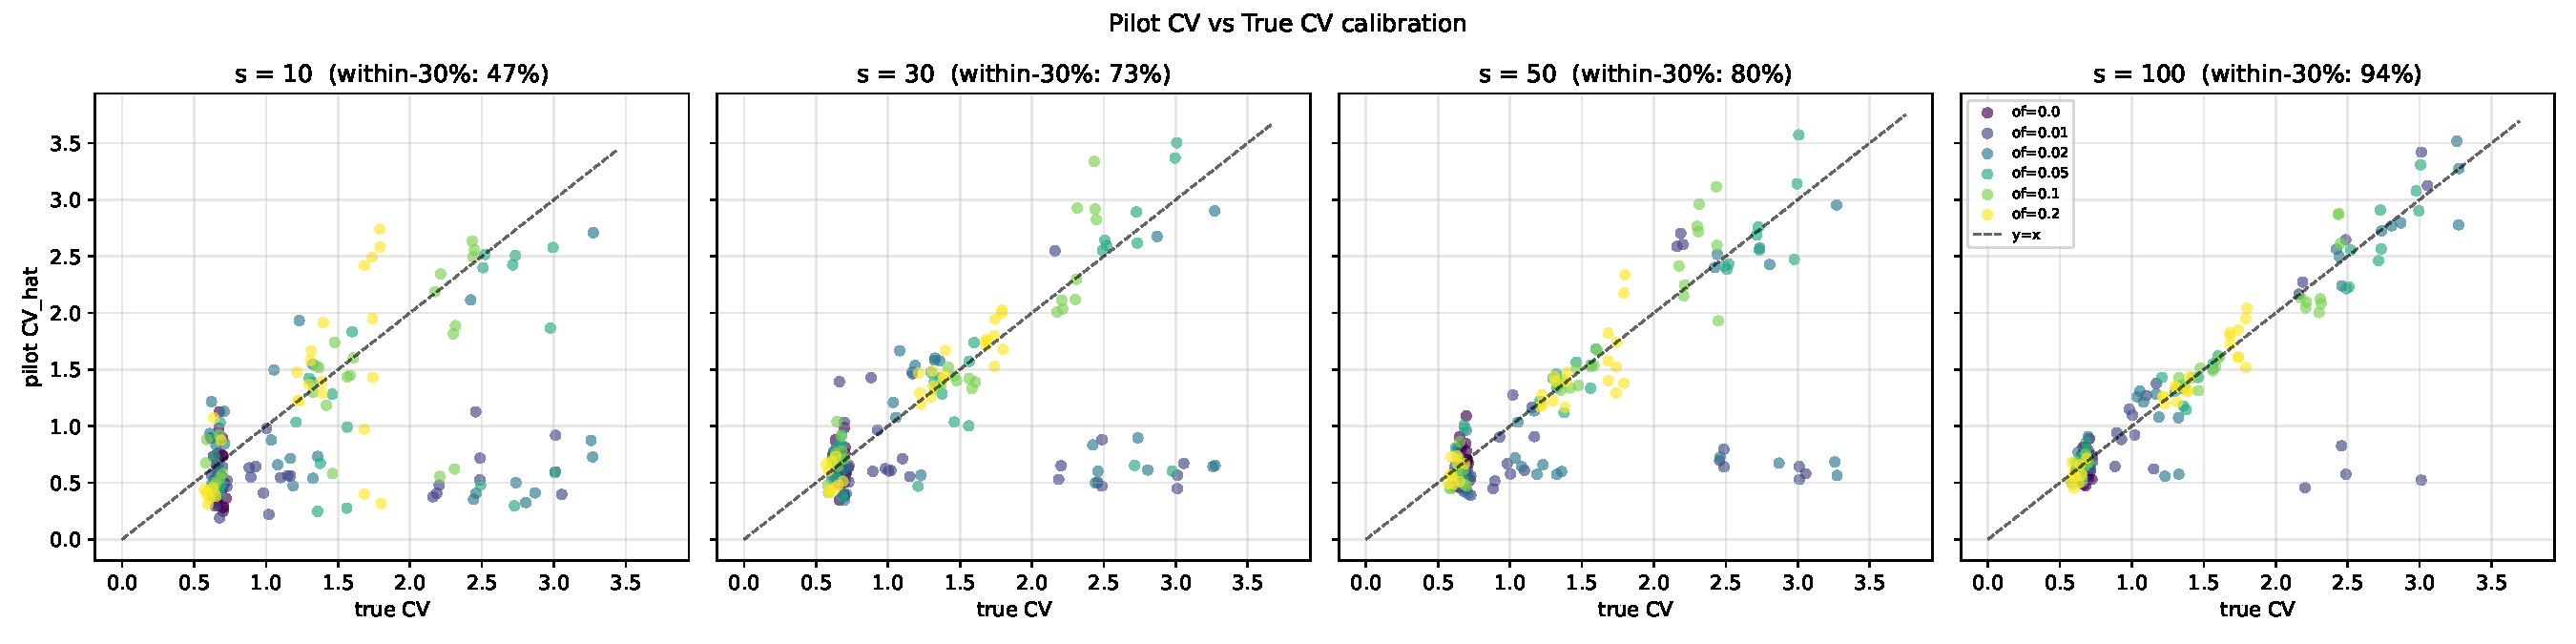
\includegraphics[width=\columnwidth]{images/fig_cv_calibration.pdf}
\caption{Pilot $\widehat{\mathrm{CV}}_s$ versus true
$\mathrm{CV}(\gamma)$ on the $162$-instance benchmark, for
$s \in \{10,30,50,100\}$. The dashed diagonal is perfect calibration.
Larger pilots concentrate more tightly around the diagonal, while
heavy-tailed instances remain systematically downward-biased because the
pilot often misses part of the tail mass.}
\label{fig:cv-calibration}
\end{figure}

The calibration improved monotonically with pilot size. Using the
headline metric
$\left|\widehat{\mathrm{CV}}_s - \mathrm{CV}(\gamma)\right| /
\mathrm{CV}(\gamma) < 0.30$, the fraction of instances within
$30\%$ of the truth was $46.91\%$ for $s=10$, $72.84\%$ for $s=30$,
$80.25\%$ for $s=50$, and $94.44\%$ for $s=100$. The corresponding
mean relative errors of $\widehat{\mathrm{CV}}_s$ were $0.370$,
$0.249$, $0.200$, and $0.119$ for $s=10,30,50,100$, while the mean
relative errors of $\widehat{M}_s$ were $0.637$, $0.466$, $0.443$,
and $0.301$. Thus, the default choice $s=50$ is already well calibrated
on most instances, while the incremental improvement from $50$ to
$100$ is noticeably smaller than the jump from $10$ to $50$.

The failure cases were not random scatter around the diagonal but
systematically downward-biased estimates on the heaviest-tailed
instances. This is consistent with the missing-mass analysis of
Section~\ref{sec:pilot-bias}: when a pilot misses a small set of large
$\gamma_a$ values, the resulting sample CV can substantially understate
the true global variability.

\subsection{Pilot Size Sensitivity}

We then measured how pilot size affects the branch decision made by
\textsc{Adaptive-Chamfer}. Using the same $162$ instances, we compared
the adaptive branch choice against the Bernstein cost-model oracle for
$s \in \{10,30,50,100\}$ and three thresholds:
$\tau = 1.5$, $\tau = \sqrt{\log n}$, and $\tau = 3.0$. The resulting
decision accuracies are shown in Figure~\ref{fig:pilot-size}. In this
accounting, the implementation's \texttt{uniform\_exact} fallback is
counted as part of the uniform side.

\begin{figure}[t]
\centering
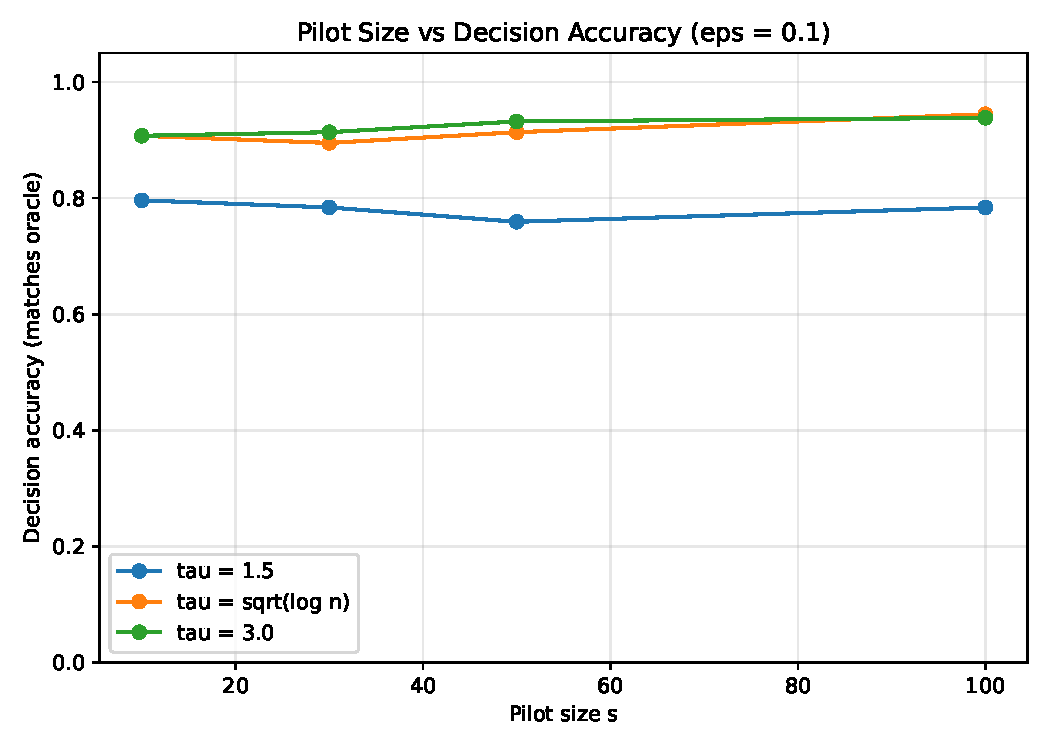
\includegraphics[width=\columnwidth]{images/fig_pilot_size.pdf}
\caption{Decision accuracy of \textsc{Adaptive-Chamfer} as a function
of pilot size $s$, measured as the fraction of benchmark instances on
which the adaptive rule selects the same branch as the Bernstein
cost-model oracle.}
\label{fig:pilot-size}
\end{figure}

At the default threshold $\tau = \sqrt{\log n}$, the decision accuracy
was $90.74\%$ for $s=10$, $89.51\%$ for $s=30$, $91.36\%$ for $s=50$,
and $94.44\%$ for $s=100$. A slightly more conservative threshold
$\tau=3.0$ performed similarly or slightly better, giving
$90.74\%$, $91.36\%$, $93.21\%$, and $93.83\%$ across the same pilot
sizes. In contrast, the more aggressive threshold $\tau=1.5$ reduced
decision accuracy to the $76$--$80\%$ range by routing too many
instances to the IS branch.

The main takeaway is that pilot size matters, but not uniformly across
all thresholds. Once the threshold is set in a reasonable range, the
decision rule is already fairly stable at $s=50$. Increasing to
$s=100$ improves accuracy further, but the gain is modest relative to
the additional pilot cost. This supports our default choice of
$s=50$ as a practical compromise.

\subsection{Threshold Sensitivity}

Fixing the pilot size at $s=50$, we next swept the threshold
$\tau$ over $20$ evenly spaced values in $[0.5, 5.0]$ and recorded
false-positive and false-negative rates relative to the Bernstein
oracle. Here a false positive means selecting IS when the oracle
prefers uniform/brute force, while a false negative means selecting
uniform when the oracle prefers IS.

\begin{figure}[t]
\centering
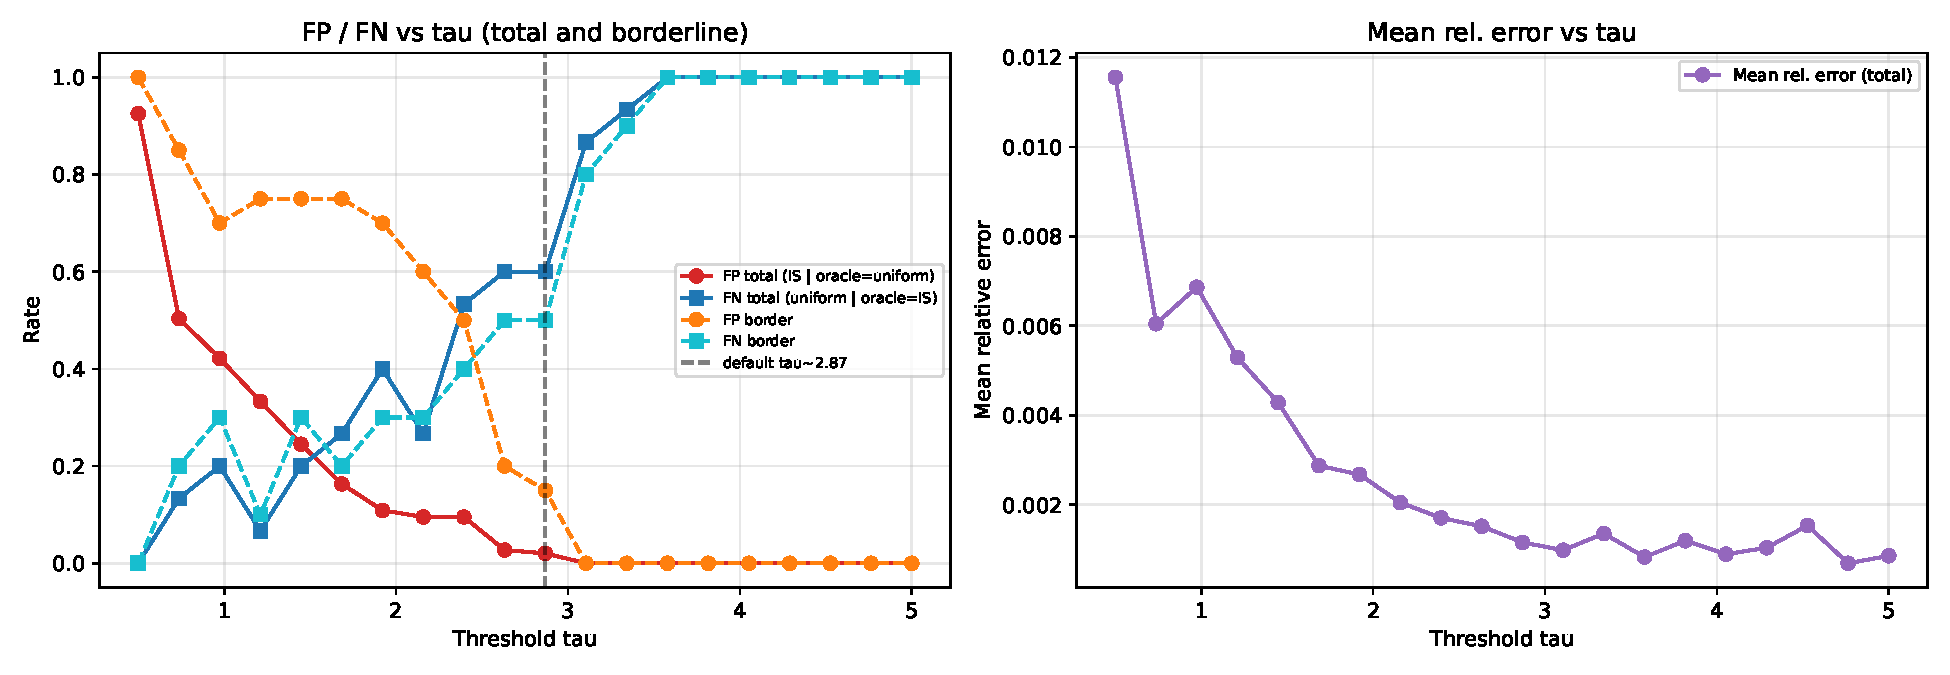
\includegraphics[width=\columnwidth]{images/fig_threshold.pdf}
\caption{Threshold sensitivity at fixed pilot size $s=50$. Left:
false-positive and false-negative rates over all instances and over the
borderline subset. Right: mean relative error as a function of the
threshold.}
\label{fig:threshold}
\end{figure}

Figure~\ref{fig:threshold} shows the expected tradeoff. Very small
thresholds over-route to IS, leading to high false-positive rates. For
example, at $\tau=0.5$ the total false-positive rate is $92.5\%$ and
the borderline false-positive rate is $100\%$. As $\tau$ increases, the
false-positive rate drops rapidly, but this comes at the cost of a
rising false-negative rate. Near the default operating point, the
closest grid value to $\sqrt{\log 2000}$ is $\tau=2.87$, where the
total false-positive rate is $2.0\%$ but the total false-negative rate
is already $60.0\%$.

This asymmetry is even clearer on the borderline subset, defined by
$\mathrm{CV}^2(\gamma) \in [0.7\log n, 1.3\log n]$. At
$\tau=2.87$, the false-positive rate on this subset is $15.0\%$, while
the false-negative rate is $50.0\%$. Thus, the pilot rule is highly
reliable on easy instances that are well away from the regime boundary,
but substantially less reliable exactly where the estimator choice is
most delicate. This finding is important for interpreting the high
overall decision accuracies of Section~\ref{sec:experiments}: those
aggregate numbers are dominated by easy cases, whereas borderline cases
remain genuinely hard.

We therefore view threshold selection as an operating-point choice
rather than a one-time calibration problem. Lowering $\tau$ suppresses
false negatives at the cost of more unnecessary IS runs; raising $\tau$
does the reverse. The current codebase uses $\tau \approx \sqrt{\log n}$
as a simple default, but Figure~\ref{fig:threshold} makes clear that no
single threshold completely resolves the ambiguity near the break-even.

\subsection{End-to-End Comparison}

Finally, we compared brute force, uniform sampling, importance
sampling, and \textsc{Adaptive-Chamfer} end-to-end on three fixed
datasets over $20$ estimator-seed trials each. Table~\ref{tab:e2e}
reports the mean relative error of the three approximate estimators and
the canonical nearest-neighbor-query-equivalent costs for the two
nontrivial routed estimators. The CSV also logs wall-clock milliseconds
from the same run, but the canonical comparison uses query-equivalent
cost because wall-clock timing is more implementation and machine
dependent.


\begin{table}[t]
\centering
\caption{End-to-end comparison. Errors are mean relative errors; costs
are nearest-neighbor-query equivalents.}
\label{tab:e2e}
\scriptsize
\setlength{\tabcolsep}{2pt}
\begin{tabular}{lccccc}
\hline
Dataset & Uniform err & IS err & Adaptive err & IS cost & Adaptive cost \\
\hline
ShapeNet-like & $0.428$ & $\mathbf{0.0118}$ & $0.0126$ & $3604$ & $5559$ \\
Text-like & $0.00291$ & $\mathbf{0.00137}$ & $0.00337$ & $3138$ & $50$ \\
Outlier & $0.384$ & $\mathbf{0.00493}$ & $0.474$ & $2771$ & $170$ \\
\hline
\end{tabular}
\end{table}

The three rows illustrate three distinct regimes. On the low-CV
Text-like dataset, the Bernstein oracle correctly prefers the uniform
path, and the adaptive estimator chooses uniform on all $20$ trials. Its
error and query-equivalent cost are therefore close to those of pure uniform sampling,
which is the intended low-variance behavior. In query-equivalent cost,
adaptive costs $50$ nearest-neighbor queries, compared with $3138$ for
the full IS pipeline. The branch counts are Uniform / IS /
Uniform-Exact $= 20 / 0 / 0$.

On the ShapeNet-like end-to-end dataset, the true CV is $3.37$, making
it a high-heterogeneity point-cloud setting, and the Bernstein oracle
prefers IS. The adaptive procedure is oracle-correct on only
$40\%$ of trials if branch correctness is scored literally, because
several runs enter the \texttt{uniform\_exact} fallback rather than the
IS branch. Its end-to-end estimation error is close to the pure-IS
error but not lower: $1.26\%$, compared with $1.18\%$ for IS and
$42.76\%$ for fixed-budget uniform sampling. In branch-count terms,
adaptive selected Uniform / IS / Uniform-Exact
$= 5 / 8 / 7$. In query-equivalent cost, adaptive costs $5559$
nearest-neighbor queries, compared with $3604$ for IS, because the
exact fallback is triggered on $7/20$ trials. This is a useful reminder
that in the small-$n$ regime, exact computation can remain competitive
even when the asymptotic theory favors IS.

The Outlier row should not be read as either simple adaptive success or
simple adaptive failure. The Bernstein oracle labels the
uniform/brute-force side as cheaper at $n=1000$, and adaptive follows
that side in all $20$ trials. Nevertheless, the adaptive run does not
reach the exact fallback; the branch counts are Uniform / IS /
Uniform-Exact $= 20 / 0 / 0$. It therefore takes a small uniform sample
and often misses the dominant point, producing $47.45\%$ mean relative
error, worse than the fixed uniform estimator's $38.38\%$. By contrast,
IS estimates the instance accurately, with $0.49\%$ error, but has
higher query-equivalent cost, $2771$ compared with $170$ for adaptive.
The result is a missing-mass failure of sample-based uniform estimation,
not an oracle-routing failure.

Overall, Table~\ref{tab:e2e} supports a nuanced conclusion. The
adaptive rule behaves exactly as intended on low-CV data, is highly
competitive on high-heterogeneity ShapeNet-like data, and cleanly exposes the
limitations of pilot-based routing on extreme heavy-tail instances.



\section{Discussion and Limitations}
\label{sec:discussion}

The main limitation of the pilot-based approach is that the pilot only
sees what it samples. When the distribution of nearest-neighbor
distances is heavy-tailed, a small pilot can entirely miss the part of
the support that makes uniform sampling unattractive. This appears both
in the calibration experiment, where heavy-tailed instances are
systematically downward-biased in Figure~\ref{fig:cv-calibration}, and
in the end-to-end Outlier row of Table~\ref{tab:e2e}, where the pilot
misses the dominant outlier with high probability and therefore has
little information about the tail. This is not a numerical bug but a
statistical limitation of any decision rule based on a small uniform
pilot.

A second limitation is that the regime boundary is genuinely ambiguous
on borderline instances. The threshold sweep in
Figure~\ref{fig:threshold} shows that high overall decision accuracy can
coexist with poor performance on the subset where
$\mathrm{CV}^2(\gamma) \approx \log n$. In other words, the pilot rule
is best understood as a coarse routing heuristic that performs well on
easy inputs, not as a sharp classifier of the exact break-even surface.
This suggests that a stronger adaptive rule may need more than a single
scalar statistic such as $\widehat{\mathrm{CV}}_s$. One natural next
step is a two-statistic rule combining $\widehat{\mathrm{CV}}_s$ with a
pilot estimate of the max-to-mean ratio $M$, which is already logged by
the current implementation.

A third limitation is computational rather than statistical. Even after
vectorization, \textsc{CrudeNN} remains the dominant engineering
bottleneck on the IS path. Our implementation is sufficient for a
course-scale empirical study, but a production implementation would
likely move the hash construction and collision checks into a compiled
backend such as Cython, Numba, or C++.

These limitations do not undercut the main contribution of the paper.
Our estimator does not improve the asymptotic complexity of Chamfer
distance estimation. Instead, it addresses a practical question left
open by prior work: when should a user pay for the IS machinery at all?
The variance analysis makes the regime boundary explicit, the
reproduction confirms the qualitative behavior of the Bakshi et al.\
estimator, and the pilot experiments show that a small automatic pilot
is often sufficient to recover the right branch in easy-to-moderate
regimes. Just as importantly, the experiments make clear where this
strategy fails: on borderline instances and on extreme heavy-tail data,
the pilot does not eliminate uncertainty so much as expose it.


\begin{thebibliography}{1}

\bibitem{bakshi2023near}
A. Bakshi, P. Indyk, R. Jayaram, S. Silwal, and E. Waingarten,
``A Near-Linear Time Algorithm for the Chamfer Distance,''
arXiv:2307.03043, 2023.
\url{https://arxiv.org/abs/2307.03043}

\bibitem{feng2025faster}
X. Feng and P. Indyk,
``Even Faster Algorithm for the Chamfer Distance,''
arXiv:2505.08957, 2025.
\url{https://arxiv.org/abs/2505.08957}

\bibitem{kusner2015wmd}
M. Kusner, Y. Sun, N. Kolkin, K. Weinberger,
``From Word Embeddings to Document Distances,''
ICML 2015.

\bibitem{diffcd2024}
E. H\"arenstam-Nielsen, D. P\"utzky, and B. Rieck,
``DiffCD: A Symmetric Differentiable Chamfer Distance for Neural
Implicit Surface Fitting,''
arXiv:2407.17058, 2024.
\url{https://arxiv.org/abs/2407.17058}

\bibitem{mckay1932}
A.~T. McKay,
``Distribution of the Coefficient of Variation and the Extended
`t' Distribution,''
\emph{Journal of the Royal Statistical Society},
vol.~95, no.~4, pp.~695--698, 1932.

\bibitem{vangel1996}
M.~G. Vangel,
``Confidence Intervals for a Normal Coefficient of Variation,''
\emph{The American Statistician},
vol.~50, no.~1, pp.~21--26, Feb.\ 1996.

\end{thebibliography}

\end{document}
